\documentclass{article}

\usepackage[margin=0.5in]{geometry}
\usepackage[czech]{babel}
\usepackage{graphicx}
\usepackage[texMathDollars]{markdown}

\begin{document}

\begin{center}
  \Large \bfseries
Ostrovní biogeografie (R. H. Mac Arthur a E. O. Wilson)
\end{center}
\pagestyle{empty}



\begin{markdown}
 
Uvažujme ostrov, na který mohou z pevniny migrovat nové druhy, které na ostrově dosud nežijí.

# Předpoklady

* Rychlost kolonizace, tj. počet druhů, které v čase
$t$ proniknou na ostrov a úspěšně se zde zabydlí, roste s počtem
imigrantů a klesá s počtem druhů, které na ostrově  již žijí.
    - První
  předpoklad je zcela přirozený.
    - Druhý předpoklad vyjadřuje v ekologii obvyklé
tvrzení, že komplexnější společenstva organismů jsou stabilnější a lépe
odolávají invazi nových druhů.
    - Předpoklad, že počet imigrantů klesá s rostoucí
vzdáleností ostrova od pevniny, což je opět přirozený  předpoklad.
    - Uvedené předpoklady splňuje funkce
$$
 \frac b{D(N+\beta)},
$$
kde $N$ je počet druhů na ostrově v čase $t$, $D$ je vzdálenost ostrova od
pevniny, $\beta$ je nezáporná a  $b$ kladná konstanta. 
* Rychlost vymírání  druhů, které v minulosti již úspěšně
kolonizovaly ostrov, ale neobstály v konkurenci pozdějších kolonizátorů,
roste s klesající rozlohou ostrova a s rostoucím počtem druhů na
ostrově.
    * Tento předpoklad
je opět přirozený, vzhledem k tomu, že ostrov menší rozlohy má menší nosnou
kapacitu.
    * Rychlost vymírání druhů je možné modelovat funkcí
$$
 a\frac {N^k}S,
$$
kde $S$ je rozloha ostrova a $a$ a $k$ jsou kladné konstanty.

# Model

Počet druhů na ostrově rozlohy $S$ ve
vzdálenosti $D$ od pevniny vyhovuje diferenciální rovnici
$$
  \frac{\mathrm dN}{\mathrm dt}= \frac b{D(N+\beta)}-a\frac {N^k}S.
$$
Předpokládáme-li, že na počátku byl ostrov neosídlený, připojíme
podmínku $N(0)=0$.

# Výstupy modelu

\end{markdown}

\begin{minipage}[t]{0.5\linewidth}
  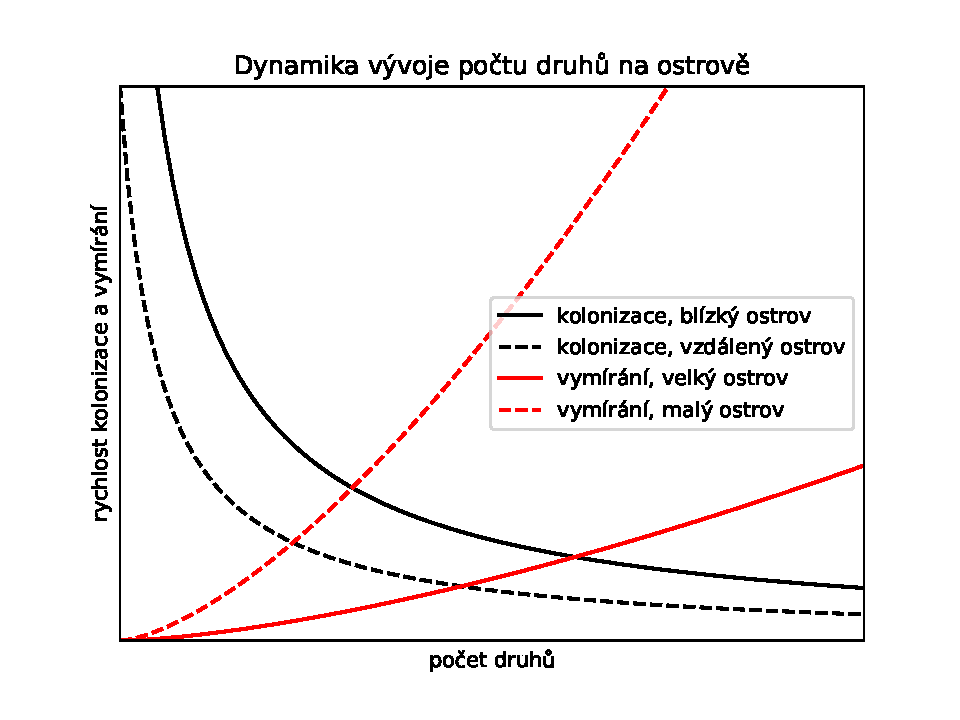
\includegraphics[width=\linewidth]{ostrov1.pdf}
\end{minipage}\begin{minipage}[t]{0.5\linewidth}
  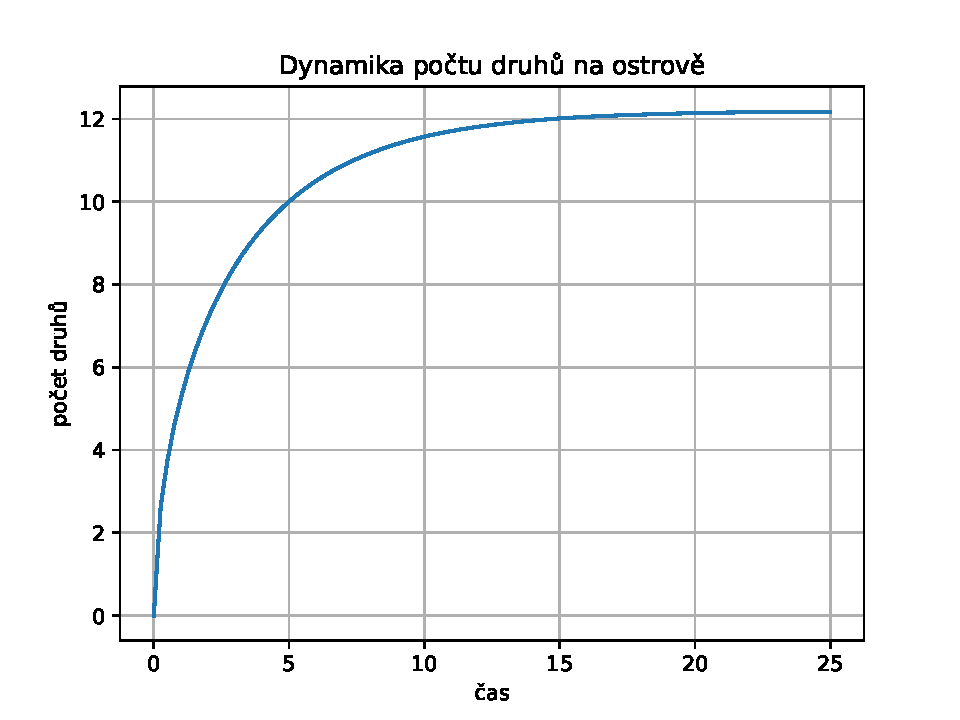
\includegraphics[width=\linewidth]{ostrov2.pdf}
\end{minipage}
\end{document}


%%% Local Variables: 
%%% TeX-command-extra-options: "-shell-escape"
%%% End: